\documentclass[11pt,a4paper]{article}
\usepackage[utf8]{inputenc}
\usepackage[T1]{fontenc}
\usepackage[polish]{babel}
\usepackage{amsmath, amsfonts, amssymb}
\usepackage{graphicx}
\usepackage[margin=2.5cm]{geometry}
\usepackage{float} % Dla lepszego pozycjonowania rysunków [H]
\usepackage{caption} % Dla podpisów
\usepackage{indentfirst} % Wcięcie pierwszego akapitu

\title{Metody Numeryczne – Projekt 3 \\ Aproksymacja profilu wysokościowego}
\author{Matsvei Kasparovich} % Zmień na swoje imię i nazwisko
\date{\today}

\begin{document}
\maketitle
\thispagestyle{empty}
\newpage
\tableofcontents
\thispagestyle{empty}
\newpage
\setcounter{page}{1}

\section{Wstęp}
\label{sec:wstep}
Celem projektu jest zbadanie przydatności dwóch metod aproksymacji interpolacyjnej – metody wykorzystującej wielomian interpolacyjny Lagrange’a oraz metody wykorzystującej funkcje sklejane trzeciego stopnia – do odtwarzania profilu wysokościowego trasy na podstawie znajomości wysokości tylko części jej punktów. Analiza została przeprowadzona na danych rzeczywistych dla kilku tras o zróżnicowanym charakterze.

\subsection{Interpolacja wielomianowa Lagrange'a}
Interpolacja wielomianowa Lagrange'a polega na znalezieniu wielomianu stopnia co najwyżej $N-1$, który przechodzi dokładnie przez $N$ zadanych punktów węzłowych $(x_i, y_i)$. Wielomian ten dany jest wzorem:
\[ P(x) = \sum_{j=0}^{N-1} y_j L_j(x) \]
gdzie $L_j(x)$ to wielomiany bazowe Lagrange'a:
\[ L_j(x) = \prod_{m=0, m \neq j}^{N-1} \frac{x - x_m}{x_j - x_m} \]
Główną zaletą tej metody jest jej prostota koncepcyjna i gwarancja przejścia przez wszystkie węzły. Wadą jest podatność na tzw. zjawisko Rungego, czyli duże oscylacje wielomianu interpolacyjnego, szczególnie w pobliżu krańców przedziału, przy dużej liczbie równoodległych węzłów. W celu poprawy stabilności numerycznej obliczeń, dziedzina funkcji interpolowanej ($x_i$) jest przekształcana do przedziału $[0,1]$ przed wyznaczeniem wielomianu, a następnie wartości są transformowane z powrotem.

\subsection{Interpolacja funkcjami sklejanymi trzeciego stopnia}
Funkcje sklejane (ang. splines) trzeciego stopnia to funkcje kawałkami wielomianowe. Dla każdego podprzedziału $[x_i, x_{i+1}]$ pomiędzy kolejnymi węzłami definiowany jest osobny wielomian trzeciego stopnia $S_i(x)$. Wielomiany te są ze sobą "sklejane" w węzłach w taki sposób, aby cała funkcja była ciągła oraz miała ciągłe pierwszą i drugą pochodną ($C^2$).
W przypadku naturalnych funkcji sklejanych zakłada się dodatkowo, że drugie pochodne na krańcach całego przedziału interpolacji są równe zero ($S''(x_0) = 0, S''(x_{N-1}) = 0$).
Funkcje sklejane są znacznie mniej podatne na oscylacje niż globalne wielomiany interpolacyjne wysokiego stopnia i zazwyczaj dają gładsze oraz bardziej naturalnie wyglądające przybliżenia.

\section{Analiza podstawowa interpolacji wielomianowej}
\label{sec:analiza_lagrange}
Analiza podstawowa dla interpolacji wielomianem Lagrange'a polegała na zbadaniu wpływu liczby węzłów interpolacyjnych na jakość aproksymacji profilu wysokościowego. Skrypt Pythona generuje wykresy dla 4, 8, 16, 32, 64 i 128 węzłów, co powinno skutkować układem subplotów 3x2.

\subsection{Trasa: Mount Everest}
Trasa "Mount Everest" charakteryzuje się jednym, wyraźnym wzniesieniem i jest stosunkowo gładka. Wyniki interpolacji wielomianem Lagrange'a przedstawiono na Rysunku \ref{fig:lagrange_everest}.

\begin{figure}[H]
    \centering
    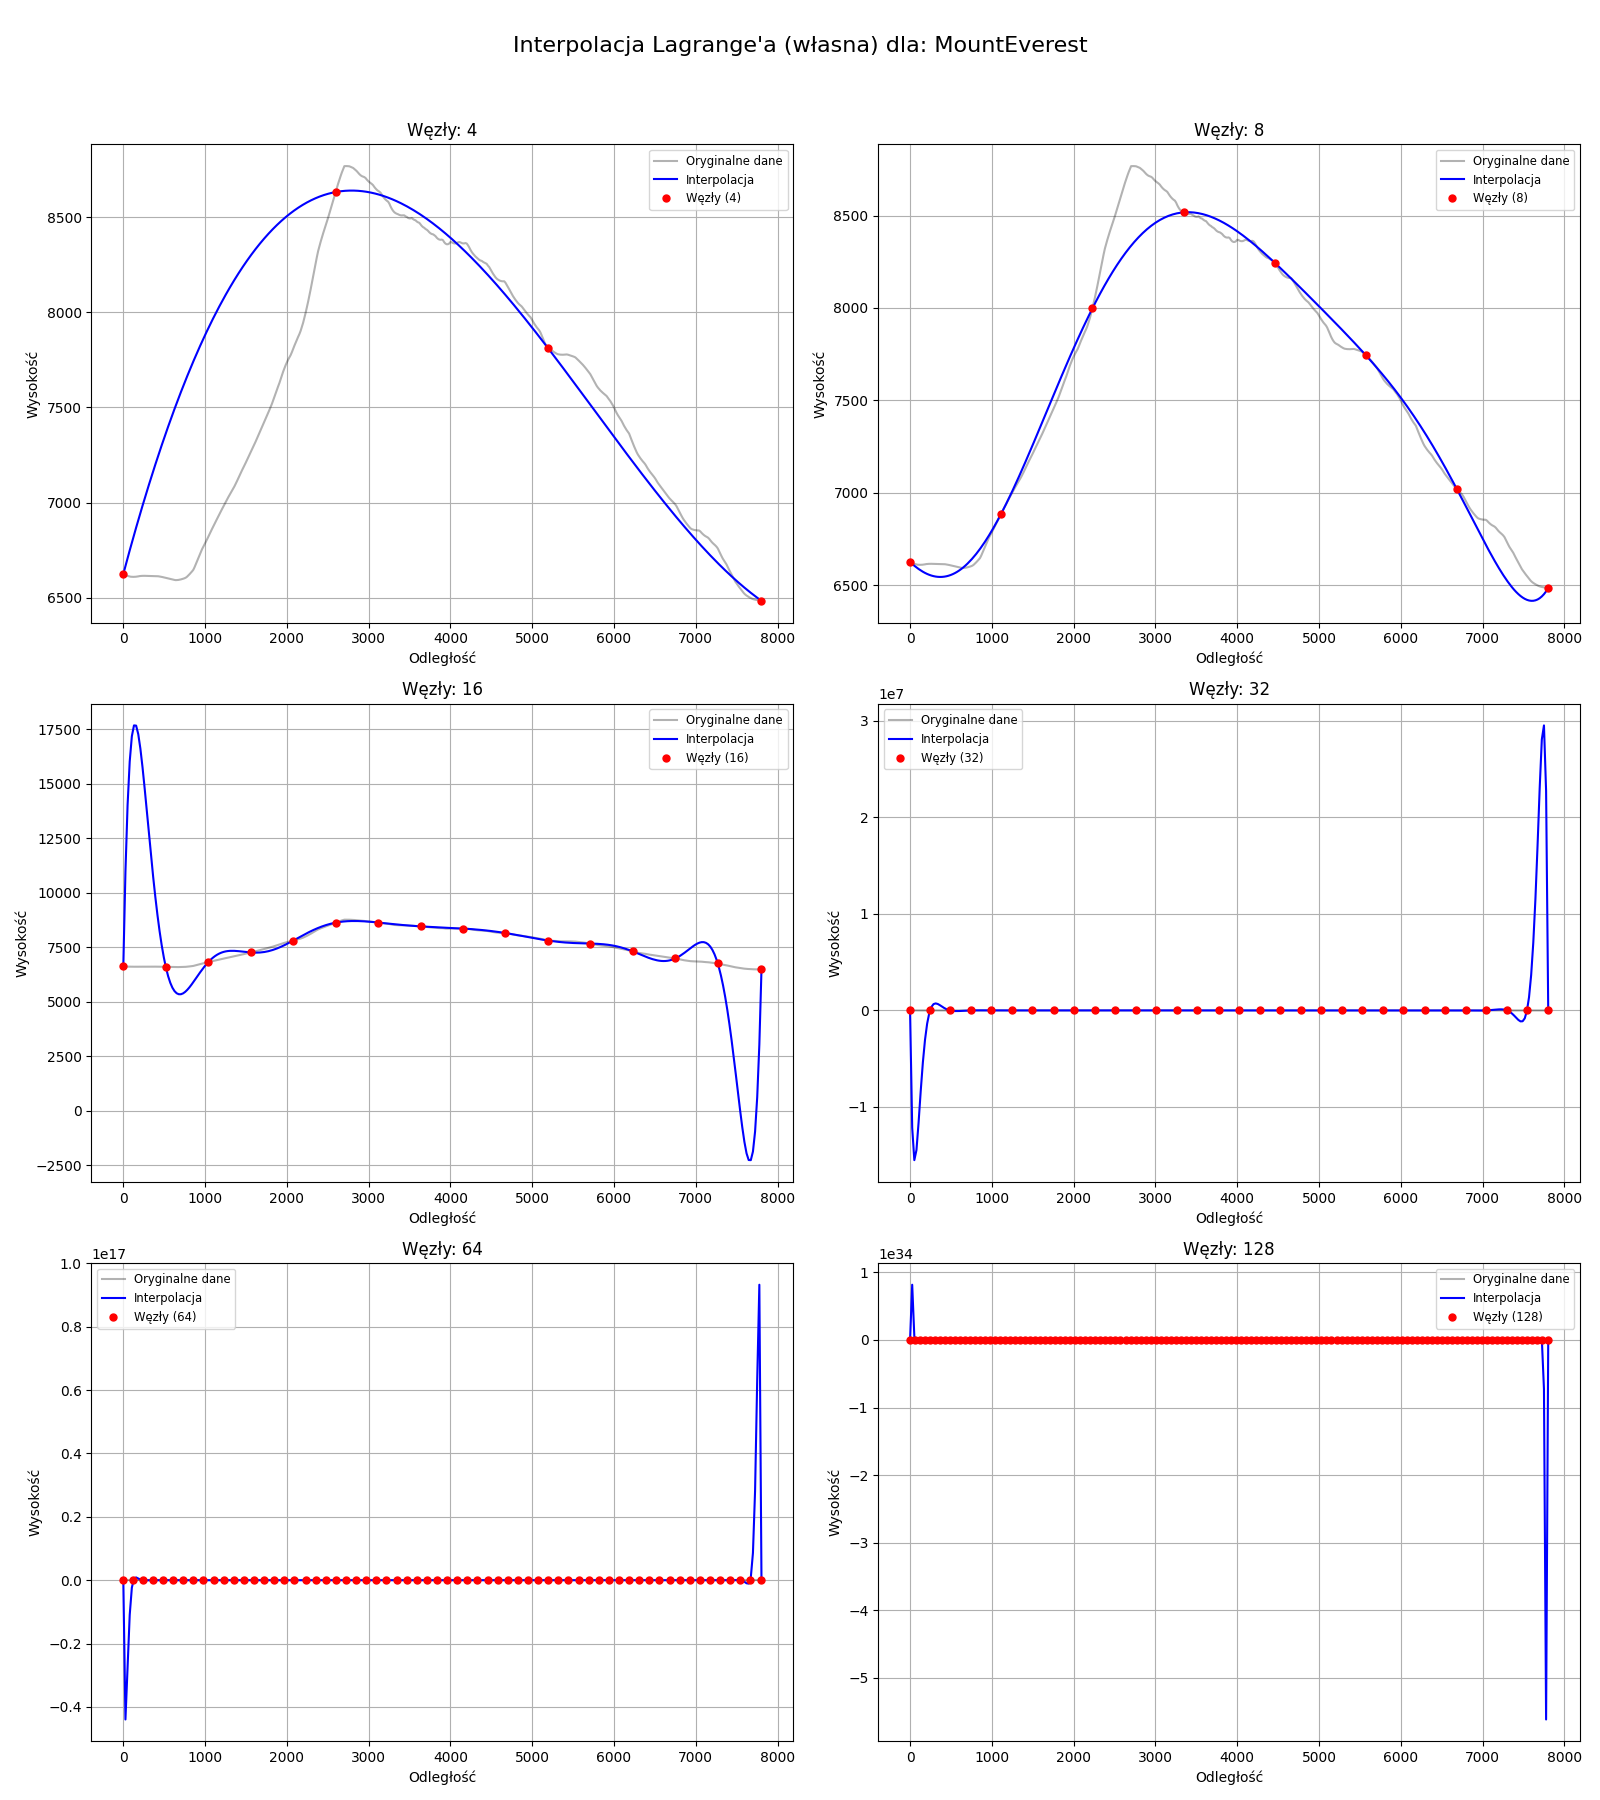
\includegraphics[width=0.95\textwidth]{MountEverest_Lagrange_basic_subplots.png} % Upewnij się, że ścieżka jest poprawna
    \caption{Interpolacja wielomianem Lagrange'a dla trasy Mount Everest przy różnej liczbie węzłów (4, 8, 16, 32, 64, 128).}
    \label{fig:lagrange_everest}
\end{figure}

\textbf{Interpretacja (Rysunek \ref{fig:lagrange_everest}):} 
\begin{itemize}
    \item \textbf{4 węzły:} Interpolacja bardzo zgrubnie oddaje ogólny kształt wzniesienia, pokazując tylko główny szczyt. Jest to bardzo uproszczony profil, bez widocznych dużych oscylacji.
    \item \textbf{8 węzłów:} Dopasowanie jest nieco lepsze, krzywa lepiej przylega do danych oryginalnych. Mogą zacząć się pojawiać niewielkie oscylacje, szczególnie na początku i końcu trasy.
    \item \textbf{16 węzłów:} Zjawisko Rungego staje się wyraźnie widoczne. Pojawiają się znaczące oscylacje, zwłaszcza na krańcach przedziału oraz w okolicach stromych zmian. Skala osi Y ulega znacznemu powiększeniu, co widać po wartościach rzędu $10^4$ do $1.75 \cdot 10^4$ przy rzeczywistym zakresie wysokości ok. 6500-8900.
    \item \textbf{32 węzły:} Interpolacja jest mocno zniekształcona przez silne oscylacje. Wyniki są nienaturalne, a skala osi Y (do $3 \cdot 10^7$) świadczy o ekstremalnie dużych wartościach interpolowanych, całkowicie odbiegających od rzeczywistości.
    \item \textbf{64 węzły:} Ekstremalne oscylacje (wartości rzędu $10^{17}$) prowadzą do wyniku całkowicie zaciemniającego rzeczywisty profil. Interpolacja jest bezużyteczna.
    \item \textbf{128 węzłów:} Wynik jest absurdalny (wartości rzędu $10^{34}$). Jest to klasyczny przykład niestabilności interpolacji Lagrange'a dla dużej liczby węzłów, z oscylacjami o rzędy wielkości przekraczającymi rzeczywisty zakres danych.
\end{itemize}
Dla trasy Mount Everest interpolacja Lagrange'a daje akceptowalne wyniki jedynie dla bardzo małej liczby węzłów (np. 4-8).

\subsection{Trasa: SpacerniakGdansk}
Trasa "SpacerniakGdansk" jest trasą względnie płaską, ale o bardziej "zaszumionym" i nieregularnym profilu. Wyniki interpolacji wielomianem Lagrange'a przedstawiono na Rysunku \ref{fig:lagrange_spacerniak}.

\begin{figure}[H]
    \centering
    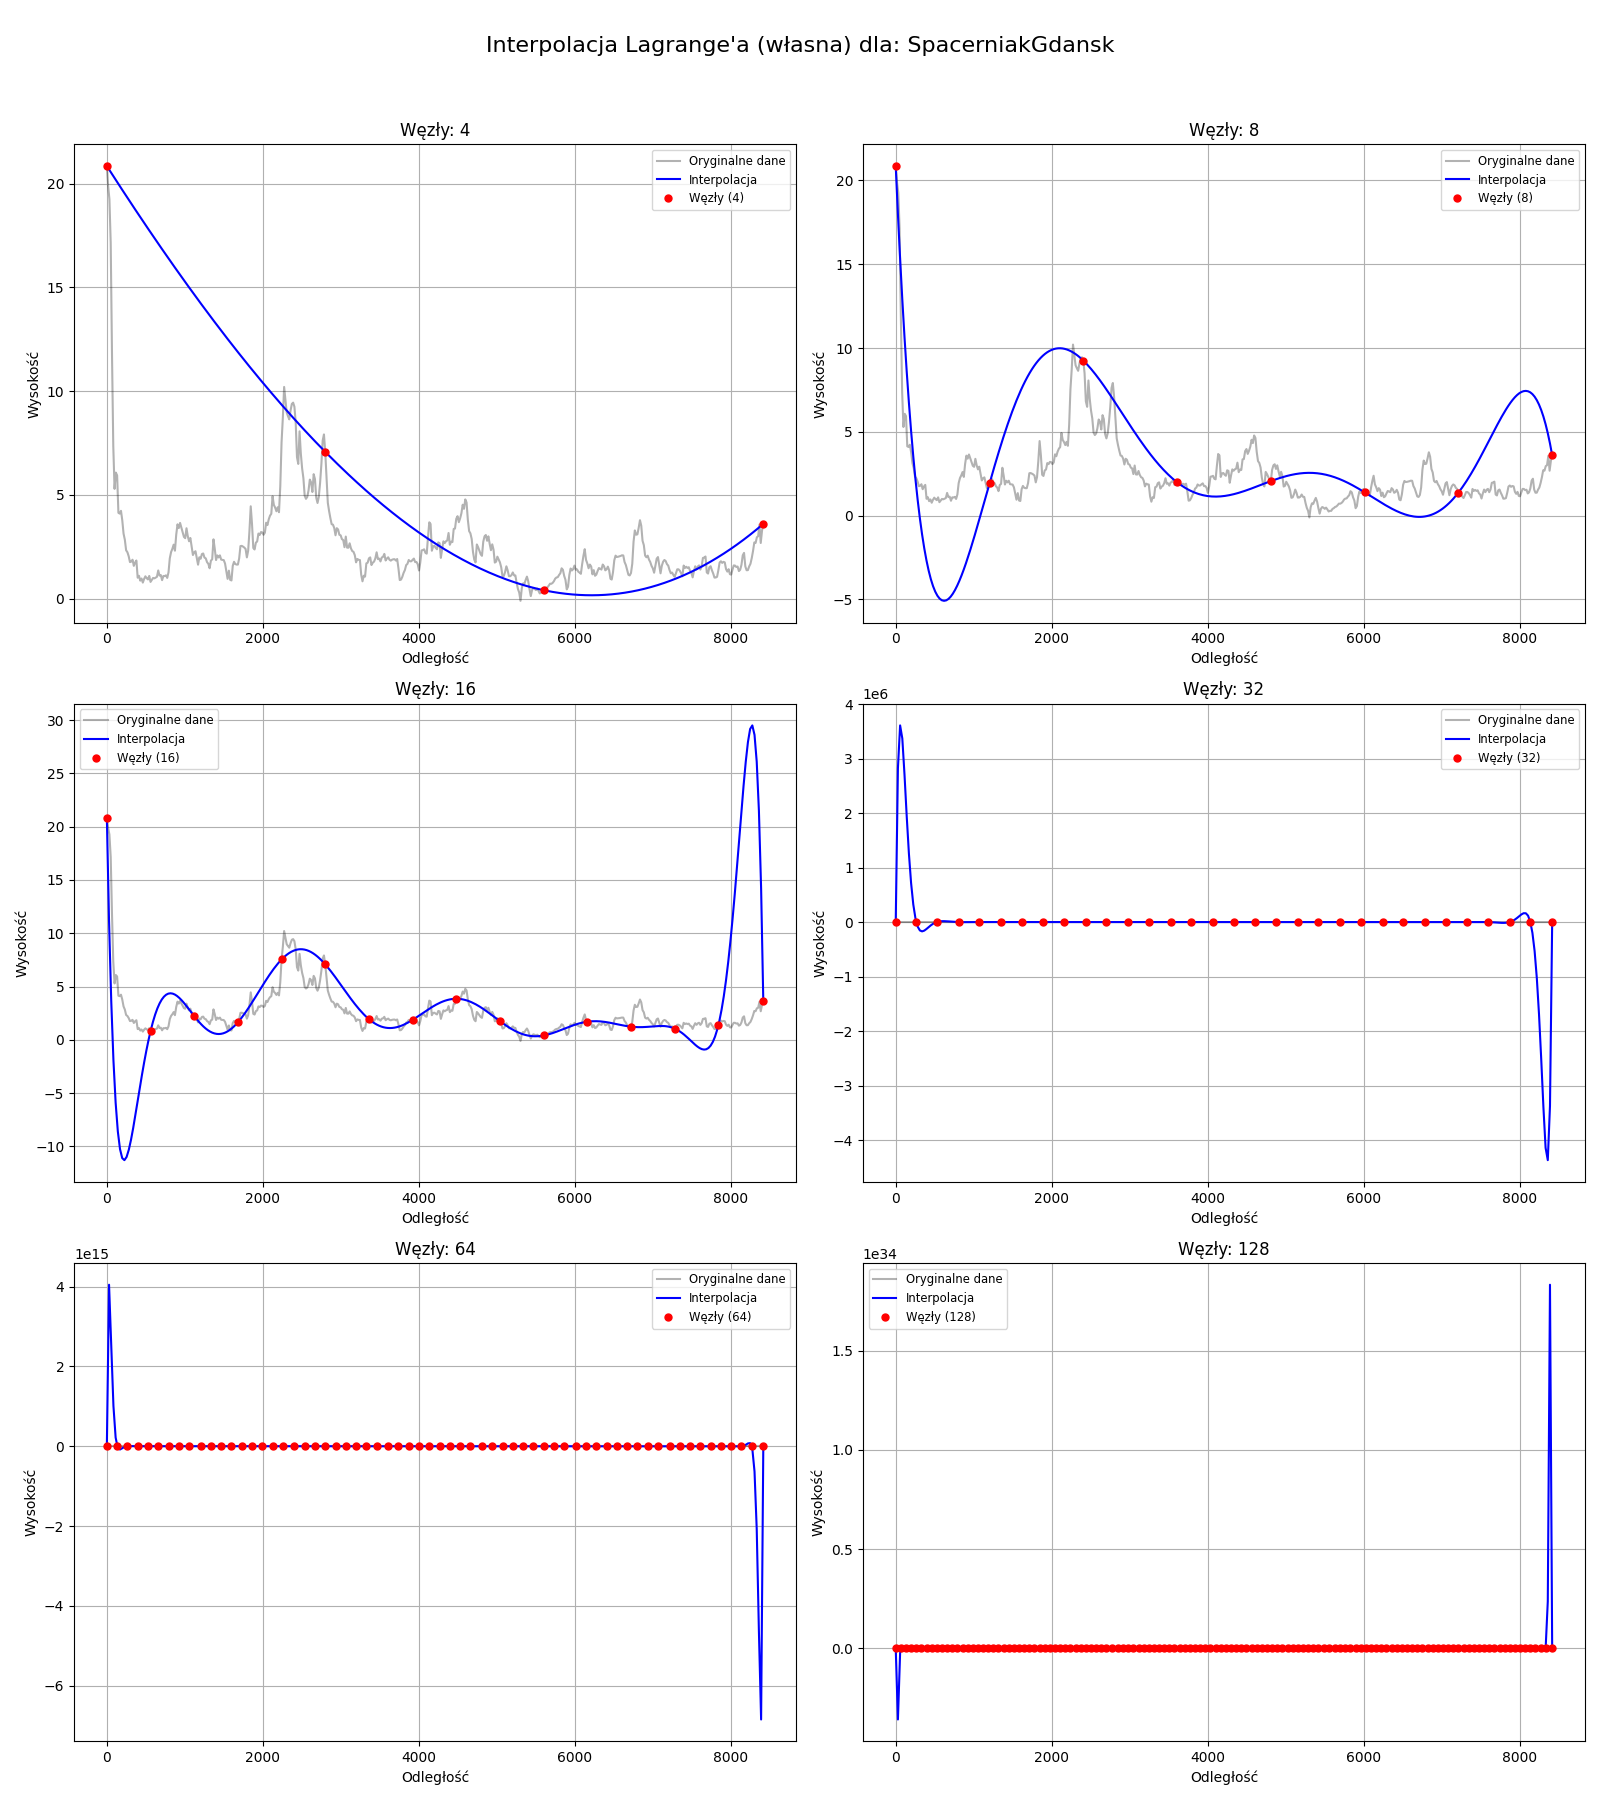
\includegraphics[width=0.95\textwidth]{SpacerniakGdansk_Lagrange_basic_subplots.png} % Upewnij się, że ścieżka jest poprawna
    \caption{Interpolacja wielomianem Lagrange'a dla trasy SpacerniakGdansk przy różnej liczbie węzłów (4, 8, 16, 32, 64, 128).}
    \label{fig:lagrange_spacerniak}
\end{figure}

\textbf{Interpretacja (Rysunek \ref{fig:lagrange_spacerniak}):} 
\begin{itemize}
    \item \textbf{4 węzły:} Interpolacja próbuje oddać ogólny, bardzo łagodny trend, ale nie jest w stanie uchwycić lokalnych zmian wysokości. Już tutaj widoczne są pewne niewielkie oscylacje, np. wartości interpolowane spadają poniżej minimalnej wysokości oryginalnej.
    \item \textbf{8 węzłów:} Oscylacje stają się bardziej zauważalne. Wielomian próbuje "dopasować się" do fluktuacji, co prowadzi do nienaturalnych wyników, np. interpolowane minimum jest znacznie niższe niż w danych oryginalnych. Skala osi Y jest już nieco większa niż rzeczywisty zakres wysokości.
    \item \textbf{16 węzłów:} Oscylacje są duże i dominują nad rzeczywistym profilem. Interpolowane wartości (np. do 30 m n.p.m. i poniżej -10 m n.p.m. przy rzeczywistym zakresie ok. 0-20 m) znacznie wykraczają poza realistyczny zakres dla tej trasy.
    \item \textbf{32 węzły:} Wynik jest bardzo zły, z ekstremalnymi wartościami (rzędu $10^6$). Interpolacja Lagrange'a kompletnie zawodzi dla tej liczby węzłów na danych o takim charakterze.
    \item \textbf{64 węzły:} Oscylacje osiągają absurdalne wartości (rzędu $10^{15}$), czyniąc interpolację całkowicie bezużyteczną.
    \item \textbf{128 węzłów:} Podobnie jak dla 64 węzłów, wynik (rzędu $10^{34}$) jest całkowicie zdominowany przez niestabilność numeryczną i zjawisko Rungego.
\end{itemize}
Dla trasy SpacerniakGdansk interpolacja Lagrange'a jest nieprzydatna praktycznie dla każdej testowanej liczby węzłów powyżej kilku najbardziej podstawowych, ze względu na szybkie pojawianie się silnych oscylacji.

\section{Analiza podstawowa interpolacji funkcjami sklejanymi}
\label{sec:analiza_spline}
Analogicznie, zbadano wpływ liczby węzłów na jakość aproksymacji profilu wysokościowego przy użyciu naturalnych funkcji sklejanych trzeciego stopnia. Skrypt Pythona generuje wykresy dla 4, 8, 16, 32, 64 i 128 węzłów.

\subsection{Trasa: Mount Everest}
Wyniki interpolacji funkcjami sklejanymi dla trasy Mount Everest przedstawiono na Rysunku \ref{fig:spline_everest}.

\begin{figure}[H]
    \centering
    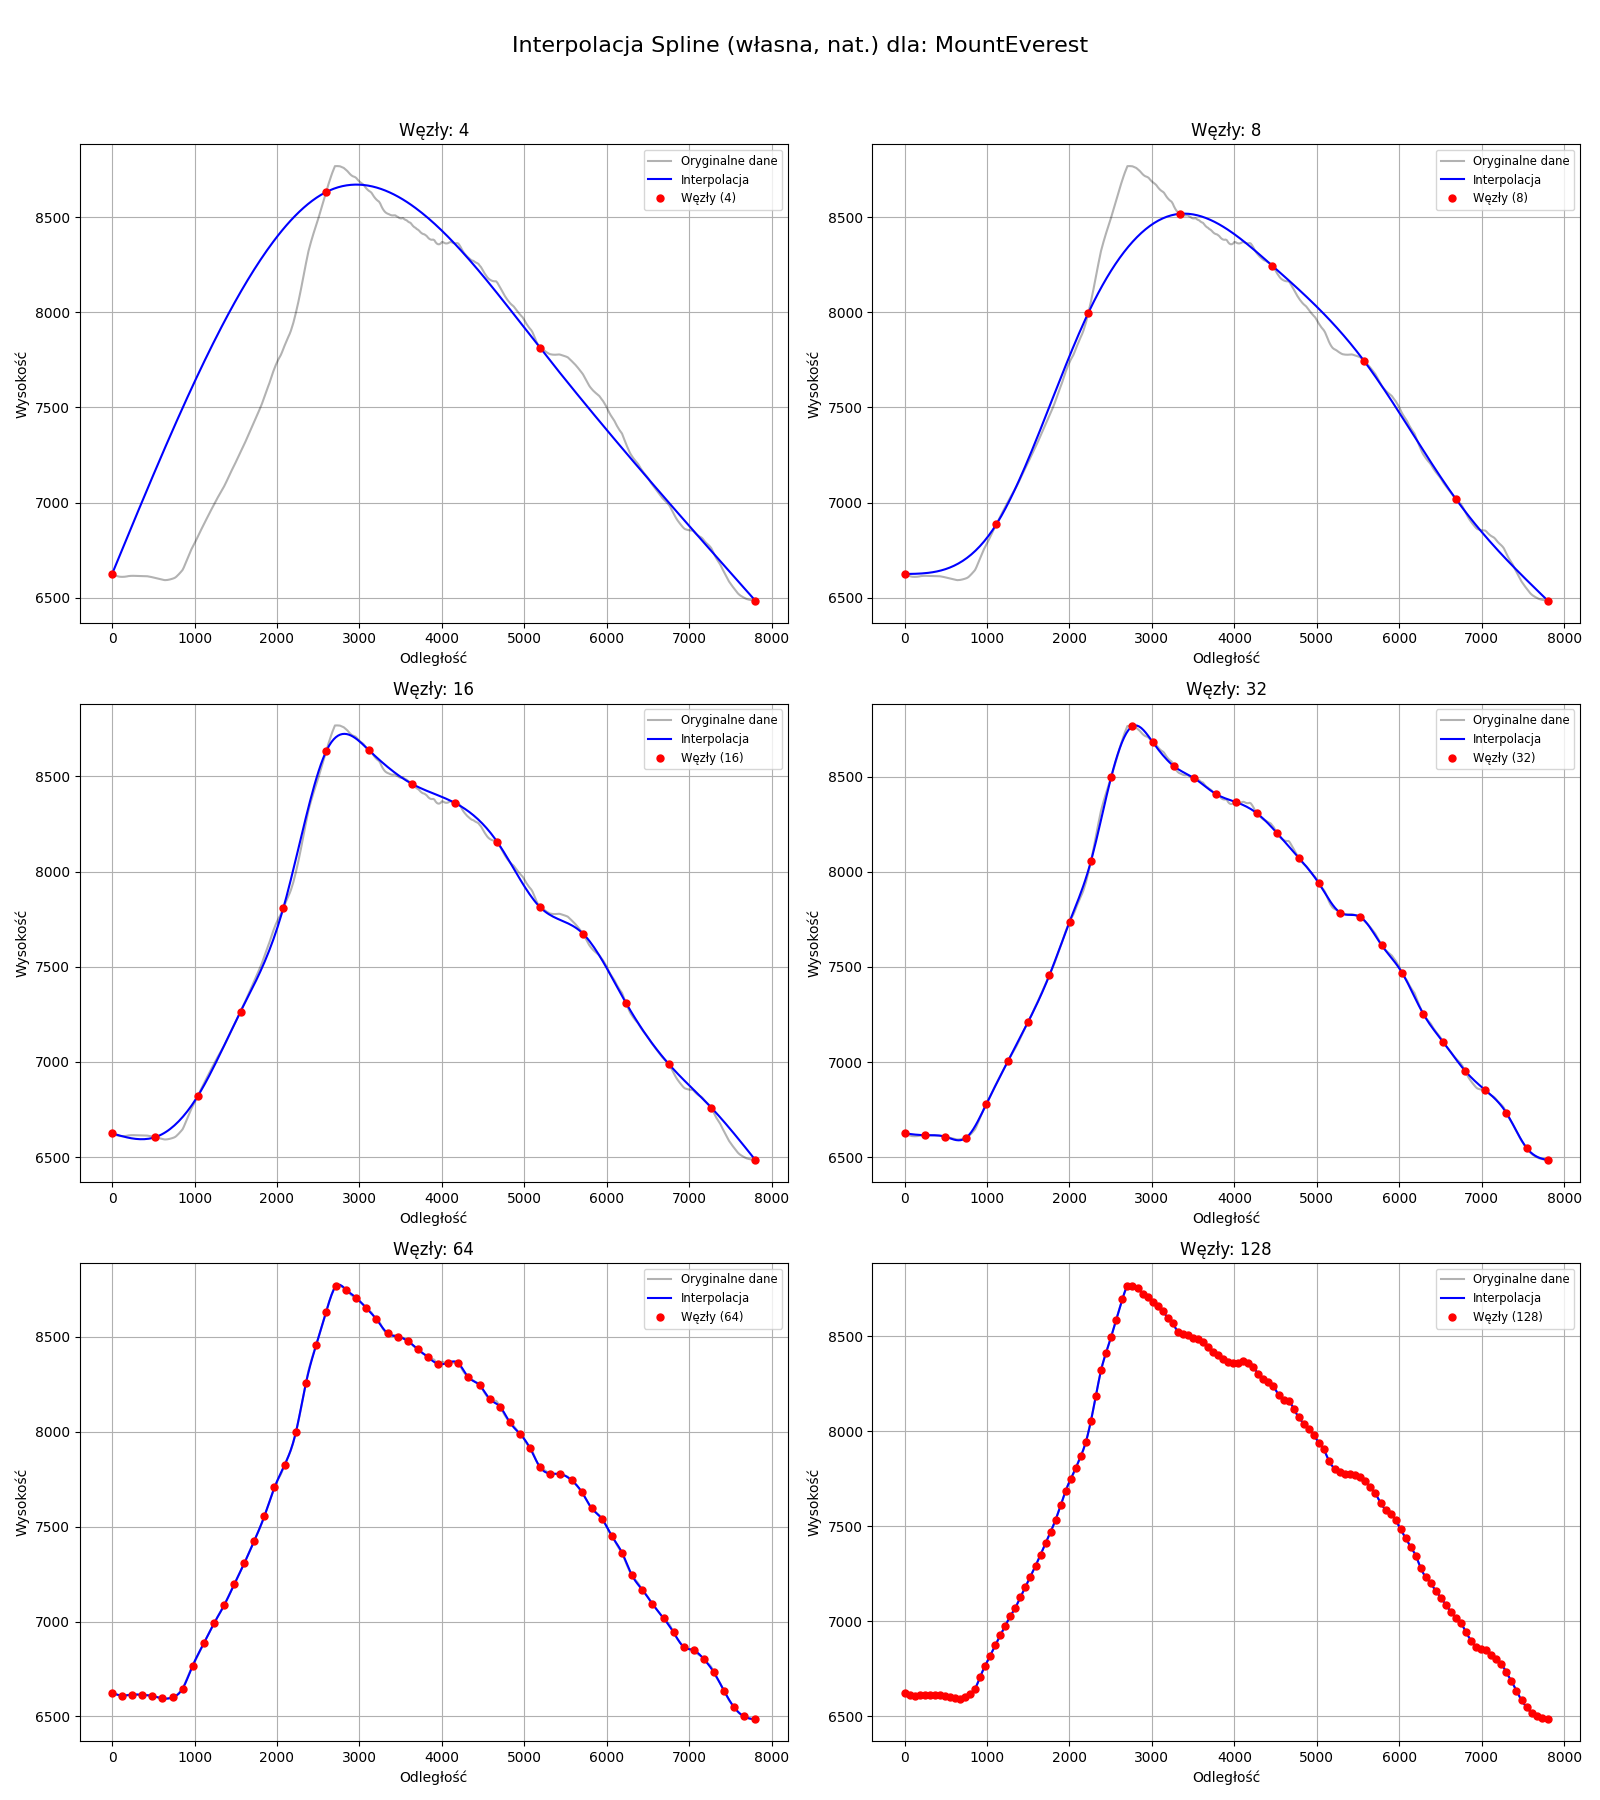
\includegraphics[width=0.95\textwidth]{MountEverest_Spline_basic_subplots.png} % Upewnij się, że ścieżka jest poprawna
    \caption{Interpolacja funkcjami sklejanymi (st. 3, naturalne) dla trasy Mount Everest przy różnej liczbie węzłów (4, 8, 16, 32, 64, 128).}
    \label{fig:spline_everest}
\end{figure}

\textbf{Interpretacja (Rysunek \ref{fig:spline_everest}):} 
\begin{itemize}
    \item \textbf{4 węzły:} Interpolacja jest gładka i dobrze oddaje ogólny kształt wzniesienia, choć z pewnymi uproszczeniami w porównaniu do danych oryginalnych.
    \item \textbf{8 węzłów:} Dopasowanie jest znacznie lepsze. Krzywa interpolacyjna gładko przechodzi przez węzły i wierniej oddaje profil trasy.
    \item \textbf{16 węzłów:} Uzyskano bardzo dobre dopasowanie. Funkcja sklejana precyzyjnie śledzi dane oryginalne, zachowując gładkość.
    \item \textbf{32 węzły:} Interpolacja jest doskonała. Krzywa niemal idealnie pokrywa się z oryginalnym profilem, bez jakichkolwiek niepożądanych oscylacji.
    \item \textbf{64 węzły:} Dopasowanie jest nadal znakomite. Krzywa interpolacyjna bardzo wiernie odwzorowuje szczegóły profilu.
    \item \textbf{128 węzłów:} Przy tak dużej liczbie węzłów, interpolacja funkcjami sklejanymi niemal perfekcyjnie odtwarza oryginalny profil, zachowując gładkość i stabilność.
\end{itemize}
Funkcje sklejane doskonale radzą sobie z interpolacją gładkiej trasy Mount Everest, a zwiększanie liczby węzłów systematycznie poprawia jakość aproksymacji.

\subsection{Trasa: SpacerniakGdansk}
Wyniki interpolacji funkcjami sklejanymi dla trasy SpacerniakGdansk przedstawiono na Rysunku \ref{fig:spline_spacerniak}.

\begin{figure}[H]
    \centering
    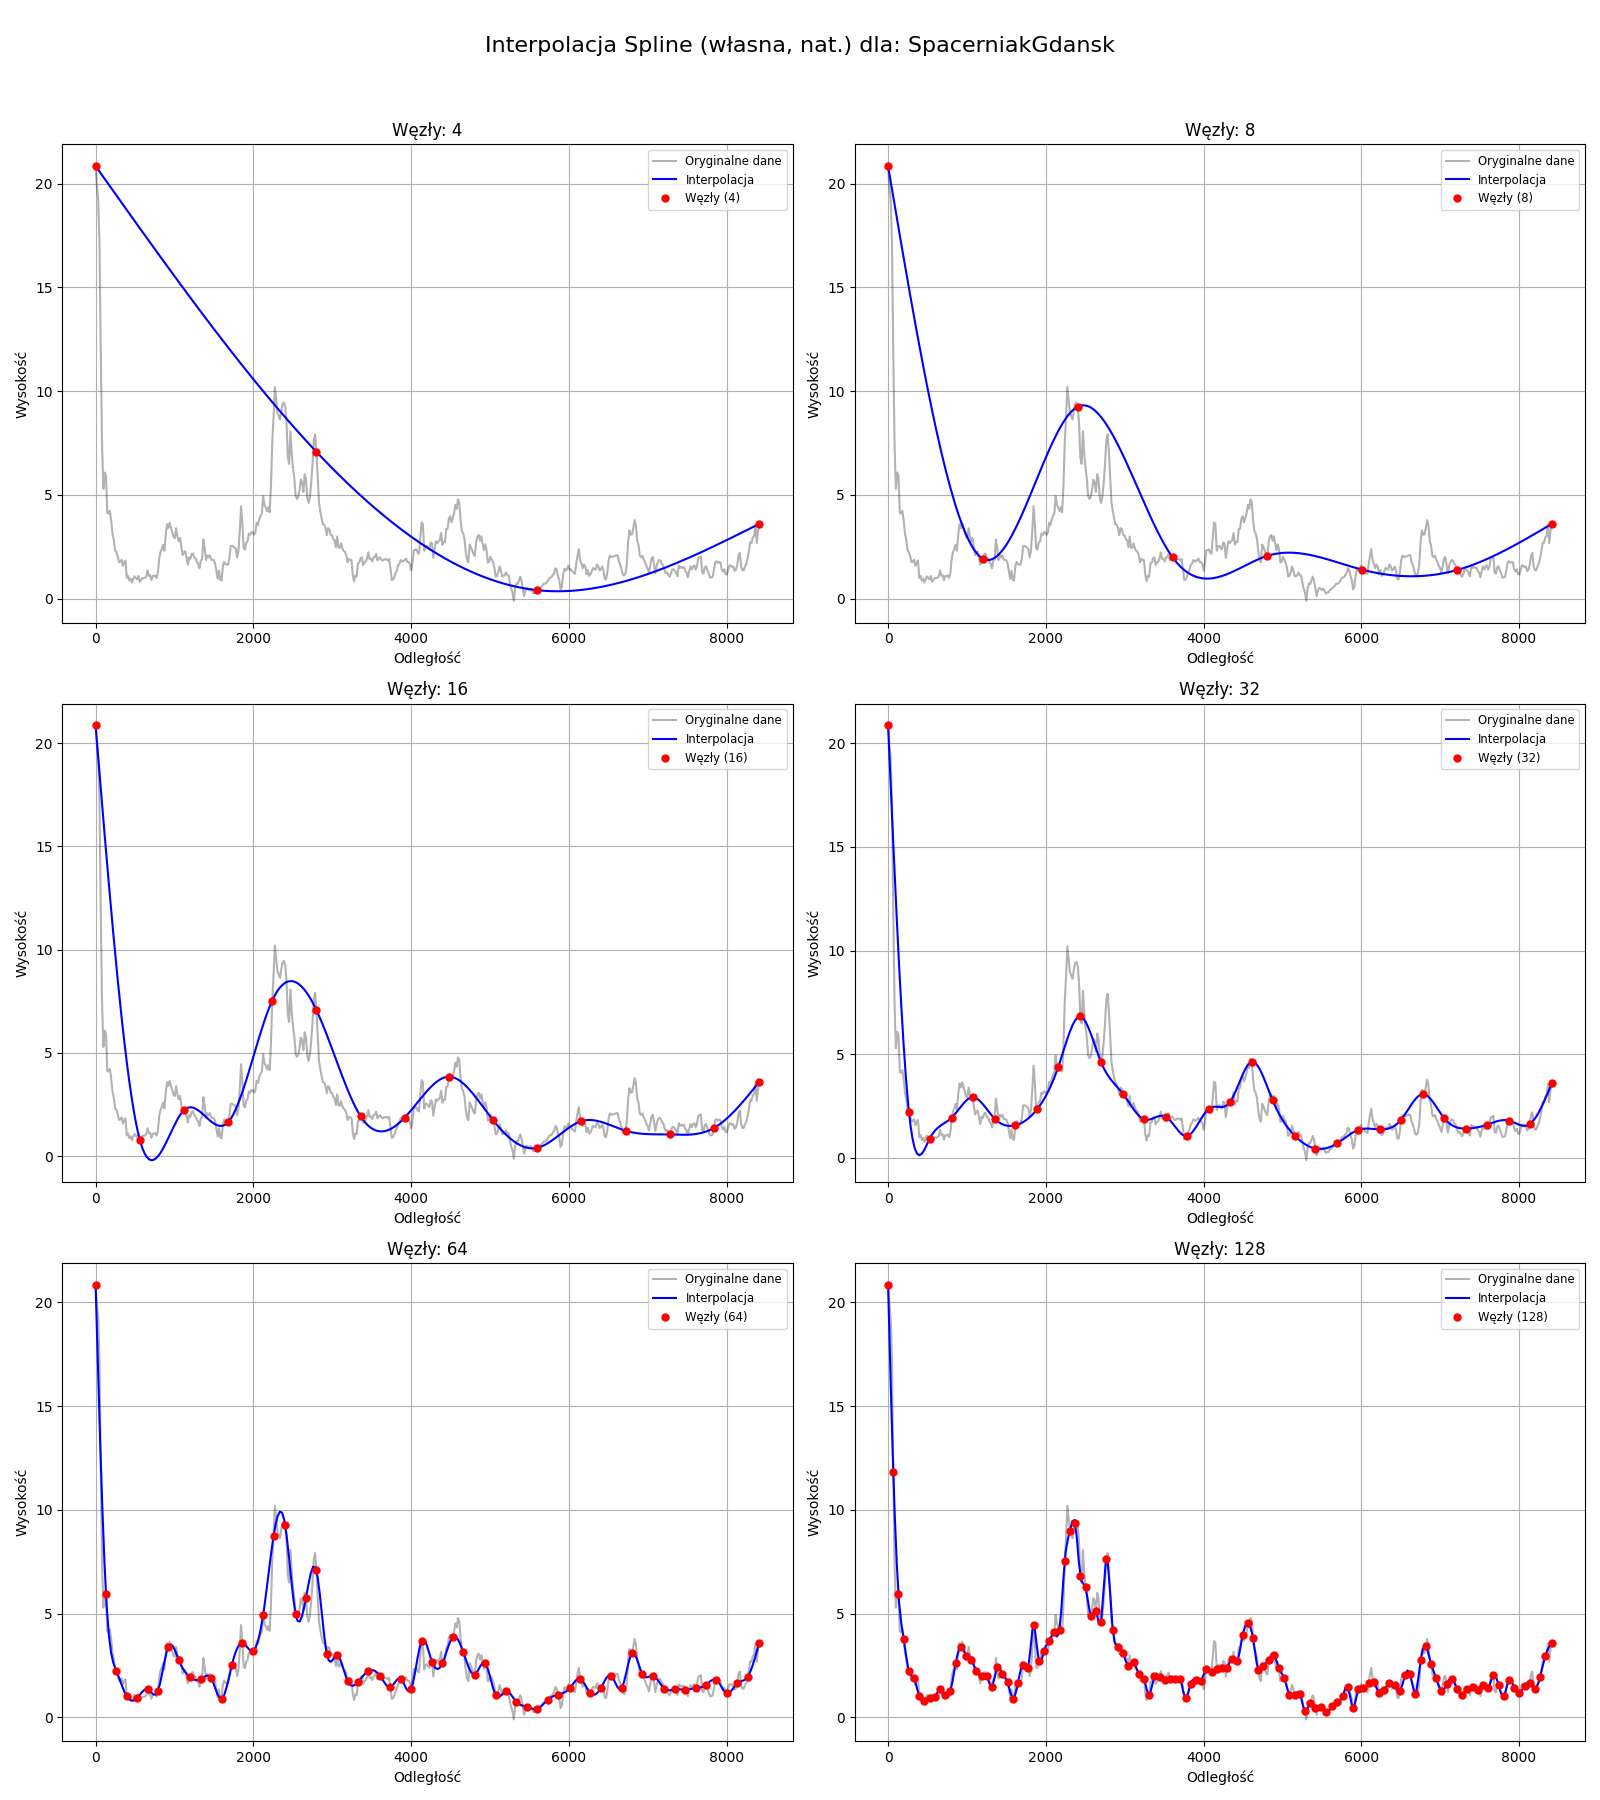
\includegraphics[width=0.95\textwidth]{SpacerniakGdansk_Spline_basic_subplots.png} % Upewnij się, że ścieżka jest poprawna
    \caption{Interpolacja funkcjami sklejanymi (st. 3, naturalne) dla trasy SpacerniakGdansk przy różnej liczbie węzłów (4, 8, 16, 32, 64, 128).}
    \label{fig:spline_spacerniak}
\end{figure}

\textbf{Interpretacja (Rysunek \ref{fig:spline_spacerniak}):} 
\begin{itemize}
    \item \textbf{4 węzły:} Interpolacja daje gładkie przybliżenie ogólnego trendu trasy, wygładzając lokalne fluktuacje.
    \item \textbf{8 węzłów:} Krzywa interpolacyjna zaczyna lepiej oddawać bardziej szczegółowe cechy profilu, nadal zachowując gładkość.
    \item \textbf{16 węzłów:} Dopasowanie jest dobre. Funkcja sklejana dobrze radzi sobie z "zaszumionym" charakterem danych, nie wpadając w oscylacje.
    \item \textbf{32 węzły:} Uzyskano bardzo dobre dopasowanie do oryginalnego, nieregularnego profilu. Funkcja jest gładka i stabilna.
    \item \textbf{64 węzły:} Dopasowanie jest jeszcze lepsze, odwzorowując drobniejsze szczegóły trasy bez utraty stabilności.
    \item \textbf{128 węzłów:} Funkcja sklejana bardzo dokładnie śledzi oryginalny, "zaszumiony" profil, demonstrując swoją wyższość nad interpolacją Lagrange'a w takich warunkach.
\end{itemize}
Interpolacja funkcjami sklejanymi jest również bardzo efektywna dla trasy SpacerniakGdansk, dostarczając stabilnych i sensownych wyników nawet przy większej liczbie węzłów i dla danych o nieregularnym charakterze.

\section{Analiza dodatkowa interpolacji: Wpływ rozmieszczenia węzłów (Węzły Czebyszewa)}
\label{sec:analiza_dodatkowa}
W ramach analizy dodatkowej zbadano wpływ nierównomiernego rozmieszczenia punktów węzłowych na jakość interpolacji wielomianem Lagrange'a. Jednym ze sposobów na złagodzenie zjawiska Rungego, które objawia się silnymi oscylacjami wielomianu interpolacyjnego (szczególnie przy równoodległych węzłach), jest zastosowanie węzłów Czebyszewa. Węzły te są zagęszczone w pobliżu krańców przedziału interpolacji, a rzadsze w jego środku. Taka dystrybucja teoretycznie minimalizuje maksymalny błąd interpolacji dla wielomianów. W praktyce, gdy węzły muszą być wybrane z istniejącego zbioru punktów danych, wybiera się punkty danych najbliższe teoretycznym węzłom Czebyszewa.

Analizę przeprowadzono dla trasy "rozne\_wzniesienia", która charakteryzuje się bardziej złożonym profilem z wieloma lokalnymi ekstremami. Zastosowano interpolację wielomianem Lagrange'a z wykorzystaniem 4, 8, 16 oraz 32 węzłów wybranych na podstawie rozkładu Czebyszewa. Wyniki przedstawiono na Rysunku \ref{fig:lagrange_chebyshev_rozne_wzniesienia}.

\begin{figure}[H]
    \centering
    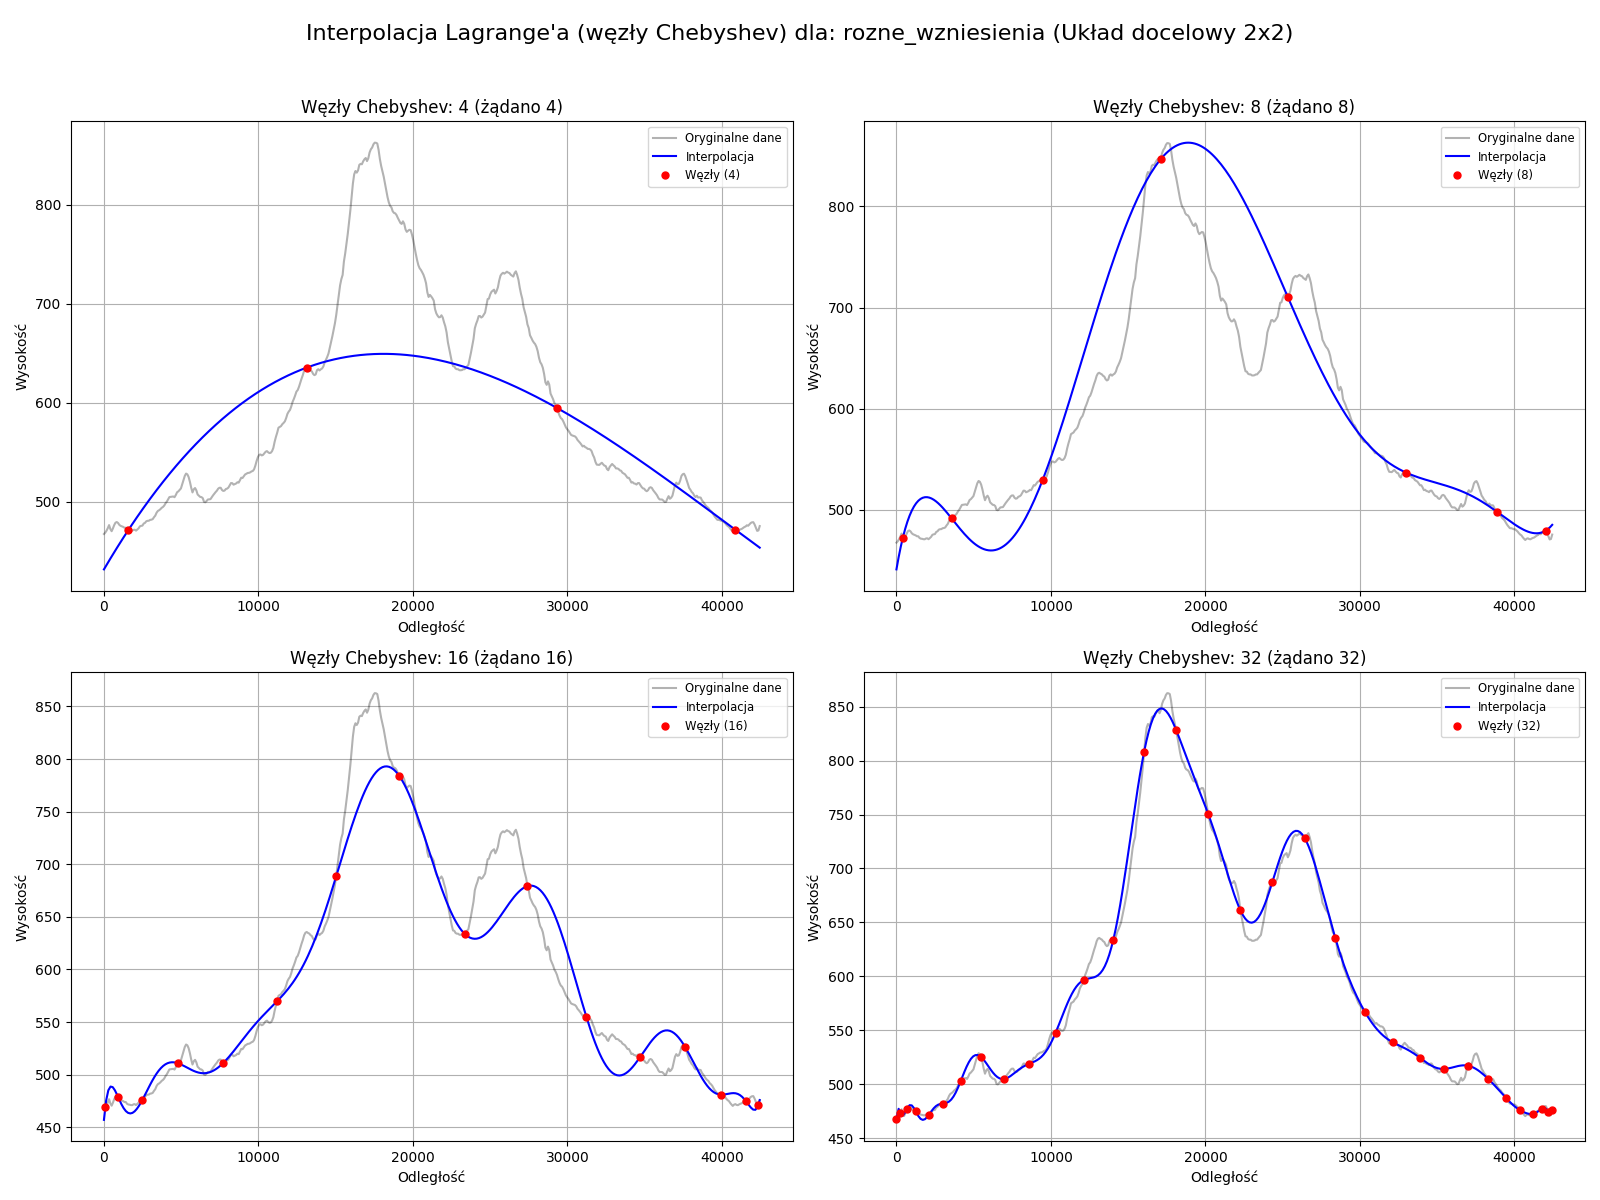
\includegraphics[width=0.9\textwidth]{rozne_wzniesienia_Lagrange_Chebyshev_2x2_subplots.png} % Upewnij się, że ścieżka jest poprawna
    \caption{Interpolacja wielomianem Lagrange'a z węzłami Czebyszewa dla trasy "rozne\_wzniesienia" przy różnej liczbie węzłów (4, 8, 16, 32). Układ docelowy 2x2.}
    \label{fig:lagrange_chebyshev_rozne_wzniesienia}
\end{figure}

\textbf{Interpretacja (Rysunek \ref{fig:lagrange_chebyshev_rozne_wzniesienia}):}
\begin{itemize}
    \item \textbf{4 węzły Czebyszewa:} Interpolacja jest bardzo gładka i oddaje jedynie ogólny zarys profilu (główne wzniesienie i spadek), pomijając większość lokalnych wzniesień i dolin. Oscylacje są minimalne, a skala osi Y (ok. 450-850) odpowiada rzeczywistemu zakresowi danych.
    \item \textbf{8 węzłów Czebyszewa:} Aproksymacja zaczyna lepiej oddawać główne cechy trasy, takie jak większe wzniesienia i niektóre doliny. Pojawiają się niewielkie oscylacje, na przykład w okolicach $x \approx 10000$ czy $x \approx 35000$, ale są one znacznie mniej wyraźne niż można by oczekiwać dla 8 równoodległych węzłów. Skala osi Y pozostaje stabilna.
    \item \textbf{16 węzłów Czebyszewa:} Wielomian interpolacyjny znacznie lepiej dopasowuje się do danych oryginalnych, odwzorowując wiele mniejszych wzniesień i dolin. Choć pewne oscylacje nadal są widoczne (np. wokół głównego szczytu czy w końcowej fazie spadku), ich amplituda jest ograniczona, a interpolacja nie wykazuje gwałtownych "wystrzałów" wartości, typowych dla zjawiska Rungego przy tej liczbie równoodległych węzłów. Skala osi Y jest zachowana.
    \item \textbf{32 węzły Czebyszewa:} Uzyskano stosunkowo dobre dopasowanie do złożonego profilu trasy. Interpolacja wiernie śledzi dane oryginalne, a oscylacje, choć obecne (np. lekkie "falowanie" wokół rzeczywistego profilu), nie zniekształcają znacząco ogólnego obrazu i nie prowadzą do absurdalnych wartości. Jest to wyraźna poprawa w stosunku do interpolacji Lagrange'a z węzłami równoodległymi, która dla 32 węzłów byłaby prawdopodobnie całkowicie bezużyteczna (por. Rysunki \ref{fig:lagrange_everest} i \ref{fig:lagrange_spacerniak}).
\end{itemize}
Zastosowanie węzłów Czebyszewa wyraźnie poprawia stabilność interpolacji wielomianowej Lagrange'a dla większej liczby węzłów, redukując problem silnych oscylacji. Chociaż interpolacja nadal może nie być tak gładka jak w przypadku funkcji sklejanych, staje się użyteczna dla większej liczby węzłów niż przy ich równomiernym rozmieszczeniu, zwłaszcza dla bardziej złożonych profili.

\section{Podsumowanie}
\label{sec:podsumowanie}
Przeprowadzona analiza podstawowa wykazała znaczące różnice w przydatności obu metod do aproksymacji profilu wysokościowego.

\textbf{Interpolacja wielomianem Lagrange'a} okazała się metodą wysoce niestabilną, szczególnie przy większej liczbie równoodległych węzłów interpolacyjnych (16 i więcej w naszych testach). Zjawisko Rungego prowadzi do powstawania dużych, nierealistycznych oscylacji, które całkowicie uniemożliwiają sensowną aproksymację profilu. Metoda ta może być brana pod uwagę jedynie przy bardzo małej liczbie węzłów (np. do około 8) i dla stosunkowo gładkich profili, jednak nawet wtedy jej użyteczność jest ograniczona. Przeskalowanie dziedziny poprawia stabilność numeryczną obliczeń, ale nie eliminuje fundamentalnego problemu oscylacji przy równoodległych węzłach. Jak wykazano w analizie dodatkowej (Sekcja \ref{sec:analiza_dodatkowa}), zastosowanie węzłów Czebyszewa może znacząco zredukować te oscylacje, poprawiając wyniki dla większej liczby węzłów, choć metoda ta nadal pozostaje generalnie mniej stabilna i daje mniej gładkie wyniki niż funkcje sklejane.

\textbf{Interpolacja naturalnymi funkcjami sklejanymi trzeciego stopnia} wykazała się znacznie lepszymi właściwościami. Jest to metoda stabilna, która dostarcza gładkich i wizualnie poprawnych aproksymacji, niezależnie od liczby użytych węzłów (w testowanym zakresie od 4 do 128). Wraz ze wzrostem liczby węzłów, jakość dopasowania systematycznie rośnie, bez wprowadzania niepożądanych artefaktów. Funkcje sklejane dobrze radzą sobie zarówno z profilami gładkimi, jak i bardziej nieregularnymi.

Oceniając działanie zaimplementowanych algorytmów, można stwierdzić, że:
\begin{itemize}
    \item Implementacja interpolacji Lagrange'a poprawnie odzwierciedla matematyczne właściwości tej metody, włączając w to jej podatność na zjawisko Rungego przy węzłach równoodległych oraz poprawę stabilności przy węzłach Czebyszewa. W tym sensie "działa" zgodnie z oczekiwaniami teorii, choć jej praktyczna przydatność do tego zadania jest ograniczona w przypadku węzłów równoodległych.
    \item Implementacja naturalnych funkcji sklejanych trzeciego stopnia działa bardzo dobrze i efektywnie realizuje zadanie aproksymacji profilu wysokościowego.
\end{itemize}

Zdecydowanie rekomendowaną metodą do aproksymacji profili wysokościowych jest interpolacja funkcjami sklejanymi trzeciego stopnia, ze względu na jej stabilność, gładkość wyników i odporność na problemy występujące w interpolacji wielomianowej wysokiego stopnia. Interpolacja Lagrange'a, nawet z węzłami Czebyszewa, powinna być stosowana z ostrożnością i świadomością potencjalnych problemów z oscylacjami.

\end{document}